
\subsection{Atari Games}

We next investigate feature transfer between randomly
selected Atari games~\cite{bellemare13arcade}. This is an interesting question, because the visuals of
Atari games are quite different from each other, as are the controls
and required strategy. Though games like Pong and Breakout are
conceptually similar (both involve hitting a ball with a
paddle), Pong is vertically aligned while
Breakout is horizontal: a potentially insurmountable
feature-level difference. Other Atari game pairs have \emph{no} discernible
overlap, even at a conceptual level.

\begin{figure}[h]
  \centering
    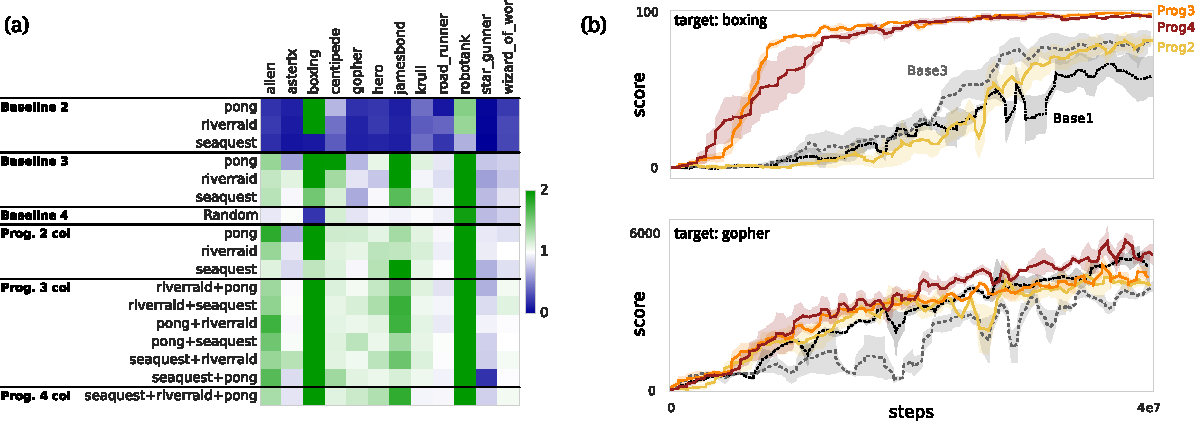
\includegraphics[width=.95\textwidth]{figures/transfer_atari.pdf}
    \caption{Transfer scores and example learning curves for Atari target games,
      as per Figure \ref{pong_results}.}
    \label{fig:atari_results}
\end{figure}

To this end we start by training single columns on three \emph{source}
games (Pong, River Raid, and Seaquest)
\footnote{Progressive columns having more than one ``source'' column are trained
sequentially on these source games, i.e.\ Seaquest-River Raid-Pong means column 1 is first trained
on Seaquest, column 2 is added afterwards and trained on River Raid, and then column 3 added and
trained on Pong.}
and assess if the learned features transfer to a different subset of
randomly selected \emph{target} games (Alien, Asterix, Boxing, Centipede,
Gopher, Hero, James Bond, Krull, Robotank, Road Runner, Star Gunner,
and Wizard of Wor). We evaluate progressive networks with 2, 3 and 4
columns, comparing to the baselines of Figure \ref{fig:baselines}).
The transfer matrix and selected transfer curves are shown in
Figure~\ref{fig:atari_results}, and the results summarized in
Table~\ref{table:main}.

Across all games, we observe from Fig.~\ref{fig:atari_results},
that progressive nets result in
positive transfer in 8 out of 12 target tasks, with only two cases
of negative transfer. This compares favourably to baseline 3, which yields
positive transfer in only 5 of 12 games. This trend is reflected in
Table~\ref{table:main}, where progressive networks convincingly outperform
baseline 3 when using additional columns. This is especially promising as
we show in the Appendix that progressive network use a diminishing amount of
capacity with each added column, pointing a clear path to online compression
or pruning as a means to mitigate the growth in model size.

Now consider the specific sequence
\textit{Seaquest}-to-\textit{Gopher}, an example of two dissimilar games. Here, the
pretrain/finetune paradigm (baseline 3) exhibits negative transfer, unlike
progressive networks (see Fig.\ref{fig:atari_results}b, bottom), perhaps
because they are more able to ignore the irrelevant features. For the sequence
\textit{Seaquest[+River Raid][+Pong]}-to-\textit{Boxing}, using additional
columns in the progressive networks can yield a significant increase in
transfer (see Fig.~\ref{fig:atari_results}b, top).

\begin{table}[t]
\begin{center}
\small
\begin{tabular}{@{}lrrrrrr@{}}
 \toprule
& \multicolumn{2}{c}{\textbf{Pong Soup}}
& \multicolumn{2}{c}{\textbf{Atari}}
& \multicolumn{2}{c}{\textbf{Labyrinth}}\\
                    & Mean (\%)    & Median (\%)  & Mean (\%)    & Median (\%)  & Mean (\%)     & Median (\%)  \\
 \midrule
  Baseline 1        & 100          & 100          & 100          & 100          & 100           & 100          \\
  Baseline 2        & 35           & 7            & 41           & 21           & 88            & 85           \\
  Baseline 3        & 181          & 160          & 133          & 110          & 235           & 112          \\
  Baseline 4        & 134          & 131          & 96           & 95           & 185           & 108          \\
  Progressive 2 col & 209          & 169          & 132          & 112          & \textbf{491}  & \textbf{115} \\
  Progressive 3 col & \textbf{222} & \textbf{183} & 140          & 111          & ---           & ---          \\
  Progressive 4 col & ---          & ---          & \textbf{141} & \textbf{116} & ---           & ---          \\

 \bottomrule
\end{tabular}
\end{center}
\caption{Transfer percentages in three domains. Baselines are defined in
    Fig.~\ref{fig:baselines}.}
\label{table:main}
\end{table}
